% Vorlage für eine Bachelorarbeit - 2012-2013 Timo Bingmann

% Dies ist nur eine Vorlage. Strikte Vorgaben wie die Bachelorarbeit auszusehen
% hat gibt es nicht. Darum können auch alle Teile angepasst werden.

%\documentclass[12pt,a4paper,twoside]{scrartcl}
\documentclass[a4paper,12pt,bibtotoc,titlepage, liststotoc,BCOR7mm,headsepline,pointlessnumbers]{scrbook}

% Diese (und weitere) Eingabedateien sind in UTF-8
\usepackage[utf8]{inputenc}

\usepackage[T1]{fontenc}
\usepackage{times}
\usepackage{float}
\typearea[current]{current}
\usepackage{fancyhdr}
\newenvironment{code}{\begingroup\footnotesize \verbatim}{\endverbatim\endgroup}

\addtokomafont{caption}{\small} % Aktive Auszeichnung von Legenden
\setkomafont{captionlabel}{\sffamily\bfseries}
%\bibliographystyle{plain}

% Sprache des Dokuments (für Silbentrennung und mehr)
\usepackage[english,german]{babel}

% Einrückung und Abstand zwischen Paragraphen
\setlength\parskip{\smallskipamount}
\setlength\parindent{0pt}

% Einige Standard-Mathematik Pakete
\usepackage{latexsym,amsmath,amssymb,mathtools,textcomp}

% Unterstützung für Sätze und Definitionen
\usepackage{amsthm}

\newtheorem{Satz}{Satz}[section]
\newtheorem{Definition}[Satz]{Definition}
\newtheorem{Lemma}[Satz]{Lemma}

\numberwithin{equation}{section}

% Unterstützung zum Einbinden von Graphiken
\usepackage{graphicx}

% Pakete die tabular und array verbessern
\usepackage{array,multirow}

% Kleiner enumerate und itemize Umgebungen
\usepackage{enumitem}

\setlist[enumerate]{topsep=0pt}
\setlist[itemize]{topsep=0pt}
\setlist[description]{font=\normalfont,topsep=0pt}

\setlist[enumerate,1]{label=(\roman*)}

% TikZ für Graphiken in LaTeX
\usepackage{tikz}
\usetikzlibrary{calc}

% Hyperref für Hyperlink und Sprungtexte
\usepackage{xcolor}

\usepackage[plainpages=false,pdfpagelabels=false,citecolor=Black, linkcolor=Black]{hyperref} %Verweise werden Links im PDF

% Paket zum Setzen von Algorithmen in Pseudocode mit kleinen Stilanpassungen
\usepackage[ruled,vlined,linesnumbered,norelsize]{algorithm2e}
\DontPrintSemicolon
\def\NlSty#1{\textnormal{\fontsize{8}{10}\selectfont{}#1}}
\SetKwSty{texttt}
\SetCommentSty{emph}
\def\listalgorithmcfname{Algorithmenverzeichnis}
\def\algorithmautorefname{Algorithmus}

\usepackage{Sweave}
\begin{document}
\Sconcordance{concordance:bachelorarbeit.tex:bachelorarbeit.Rnw:%
1 74 1 1 0 364 1 1 31 1 2 8 1 1 36 1 2 14 1 1 17 1 2 11 1 1 22 1 2 10 1 %
1 14 1 2 11 1 1 11 245809 0 1 2 6 1 1 13 483890 0 1 2 57 1}


%%%%%%%%%%%%%%%%%%%%%%%%%%%%%%%%%%%%%%%%%%%%%%%%%%%%%%%%%%%%%%%%%%%%%%

\pagestyle{empty} % keine Seitenzahlen
\renewcommand{\thepage}{\roman{page}}

% Titelblatt der Arbeit
\begin{titlepage}

  \begin{center}\large
  \begin{flushleft}
    \quad\includegraphics[height=17px]{kit_logo_de.pdf} \hfill
     
  \end{flushleft}
    %\includegraphics[height=20mm]{grouplogo-algo-blue.pdf}\quad\null

    \vfill
    \vfill
    \vfill
    \vfill

    Bachelor thesis
    \vspace*{2cm}

    {\bf\huge Title of Thesis  \par}
    % Siehe auch oben die Felder pdftitle={}
    % mit \par am Ende stimmt der Zeilenabstand

    \vfill

    Name of author

    \vspace*{15mm}

    Date: \today 

    \vspace*{40mm}
    \begin{tabular}{rl}
      Supervisors: & Prof. Dr. Peter Sanders \\
      & Dipl. Inform. Zweiter Betreuer \\
    \end{tabular}
    
    \vspace*{10mm}

    %Institut für Theoretische Informatik, Algorithmik \\
    %Fakultät für Informatik \\
    %Karlsruher Institut für Technologie

    \vspace*{10mm}
    % English:
     Institute of Theoretical Informatics, Algorithmics \\
     Department of Informatics \\
     Karlsruhe Institute of Technology

    \vspace*{12mm}
    \vfill
  \end{center}

\end{titlepage}

%%%%%%%%%%%%%%%%%%%%%%%%%%%%%%%%%%%%%%%%%%%%%%%%%%%%%%%%%%%%%%%%%%%%%%
%%%%%%%%%%%%%%%%%%%%%%%%%%%%%%%%%%%%%%%%%%%%%%%%%%%%%%%%%%%%%%%%%%%%%%

%\vspace*{0pt}\vfill
\ 
\newpage
\clearpage

\section*{Abstract}
In this thesis we augment the existing Hypergraph Partitioner KaHyPar with an evolutionary framework with the goal to improve the 
solution quality.
\addcontentsline{toc}{chapter}{Abstract}
\selectlanguage{english}
% German and English Abstract
\vfill\vfill\vfill
\ 
\newpage
\clearpage
\ 
\newpage
\clearpage

%%%%%%%%%%%%%%%%%%%%%%%%%%%%%%%%%%%%%%%%%%%%%%%%%%%%%%%%%%%%%%%%%%%%%%
\section*{Acknowledgments}

I'd like to thank Timo for the supply of Club-Mate
\vfill\vfill\vfill
Hiermit versichere ich, dass ich diese Arbeit selbständig verfasst und keine anderen, als die angegebenen Quellen und Hilfsmittel benutzt, die wörtlich oder inhaltlich übernommenen Stellen als solche kenntlich gemacht und die Satzung des Karlsruher Instituts für Technologie zur Sicherung guter wissenschaftlicher Praxis in der jeweils gültigen Fassung beachtet habe.

\bigskip
\vspace*{1cm}
\noindent
Ort, den Datum

\clearpage

%%%%%%%%%%%%%%%%%%%%%%%%%%%%%%%%%%%%%%%%%%%%%%%%%%%%%%%%%%%%%%%%%%%%%%
\tableofcontents
\clearpage
%%%%%%%%%%%%%%%%%%%%%%%%%%%%%%%%%%%%%%%%%%%%%%%%%%%%%%%%%%%%%%%%%%%%%%
\clearpage
%%%%%%%%%%%%%%%%%%%%%%%%%%%%%%%%%%%%%%%%%%%%%%%%%%%%%%%%%%%%%%%%%%%%%%
\mainmatter
\pagestyle{plain}
\chapter{Introduction}
\pagestyle{headings}
\section{Motivation}
A Hypergraph is a generalization from a regular graph in the regard that the edges may contain more than 2 vertices.
Many real world scenarios like warehouse article limits, social networks and structures like computer chips can be modeled accurately as a hypergraph but only imprecise as a graph. As a result there are many applications to partition a hypergraph into $k$ blocks in order to analyze or optimize the circumstances translated towards their respective mathematical model. The objective is to minimize the cut between the blocks. Primarily VLSI design is benefitting from hypergraph partitioning in a sense that the amount of interconnected components is bottlenecking the performance and chip size. \cite{boese1992high} The size of the components also should not be severely disproportionate as this requires longer connections between the components resulting in longer transmission times. \footnote{https://www.nobelprize.org/educational/physics/integrated_circuit/history/} Therefore the component sizes should be balanced.
When trying to maintain balance for the block size hypergraph partitioning is a problem that, similar to balanced graph partitioning, is proven to be NP-hard. \cite{garey2002computers} Since the exact calculation for NP-hard problems is not feasible using the current academic knowledge and state-of-the-art algorithms these problems are often approached using heuristics to improve the corresponding objective while having a practicable runtime. One of the most effective heuristic in regard to graph/hypergraph partitioning is the multilevel paradigm \cite{bulucc2016recent}. By reducing the hypergraph whilst maintaining the hypergraph structure the original problem is translated to an easier problem by a large margin. Therefore a strong initial solution can be created and additionally be improved on during the recreation of the original problem using local search algorithms. While this approach is capable of generating a strong solution within one execution it falls short on further improving this solution due to the limited solution space evaluated. This problem is can be counteracted using meta heuristics such as evolutionary algorithms specifically designed to allow a more efficient traversal of the solution space and avoidance of local optima. 

\section{Contribution}
This thesis will augment the existing hypergraph partitioner KaHyPar by adding an evolutionary framework designed to improve on the solution quality generated by KaHyPar. Transferring an existing evolutionary framework for graph partitioning KaffPaE, we add new operators to improve the solution quality by evaluating and modifying the structures of solutions generated by KaHyPar in a more effective manner. 
\section{Structure of Thesis}
In the beginning the main focus is to describe precisely how KaHyPar is utilizing the multilevel paradigm to generate the partitions. Afterwards the evolutionary framework is introduced, described and motivated and finally evaluated by comparing the solution quality of the evolutionary algorithm against KaHyPar by partitioning multiple instances using both variants. 
%%%%%%%%%%%%%%%%%%%%%%%%%%%%%%%%%%%%%%%%%%%%%%%%%%%%%%%%%%%%%%%%%%%%%%
\chapter{Preliminaries}
\section{General Definitions}

A Hypergraph $H = (V, E, c, w)$ is defined as a set of vertices $V$ a set of hyperedges $E$ where each edge may contain an arbitrarily large subset of $V$.

The weight of a vertex is measured by $c: V \rightarrow  \mathbb R_{\ge 0}$ a function assigning a weight value. Similarly the weight of a hyperedge is defined by $w: E \rightarrow  \mathbb R_{\ge 0}$. 
Two verticies $u, v$ are adjacent if $\exists e \in E | u, v \in e$ and a vertex $u$ is incident to a hyperedge $e$ if $ u \in e$. The size $|e|$ of an Hyperedge $e$ is the number of vertices contained in $e$. A k-way partition of a Hypergraph $H$ is a partition of $V$ into k disjoint blocks $V_1, .. V_k$. $part: V \rightarrow [0, k-1]$ is a function referencing the corresponding block of a k-way partition to a vertex $u$. 
A k-way partition is balanced when the weight of each block $V_i | 1 \le i \le k, \sum_{v_i \in V_i} c(v_i) \le (1 + \epsilon) \lceil \frac{\sum_{v \in V} c(v)}{k} \rceil $  for a balance constraint $\epsilon$.
A valid solution is a balanced k-way partition. An invalid solution is a partition where either the balance criterion is not met, or $H$ has been partitioned for a different value for k.
A Hyperedge $e$ is a cut edge $cut(e)$ if $\exists u,v \in e | part(u) \neq part(v)$. The connectivity of a Hyperedge $e$ is $\lambda(e)$ = $\sum_{i=0}^{k-1} \delta(e,i) | \delta(e, i) = 
     \begin{cases}
       \text{1} &\exists v \in e\text{ }part(v)=i\\
       \text{0} &\text{else}\\
     \end{cases}$ 

The set cut edges in H is defined as
$cut(E) := \{e \in E | cut(e) \}$.
The multiset connectivity edges in H is defined as
$conn(E) := \{a(e) \in E | cut(e) \} |a(e) := \lambda(e)$
The cut metric $cut(H) := \sum_{e \in E} 
\begin{cases}
       \text{w(e)} & \text{e is cut edge}\\
       \text{0} &\text{else}\\
     \end{cases}$  and gives the value of cuts.
The connectivity metric $(\lambda -1)(H) := \begin{cases}
       \text{$\lambda(e)*w(e)$} & \text{e is cut edge}\\
       \text{0} &\text{else}\\
     \end{cases}$
Both metrics can be used to measure the quality of a solution. Throughout this thesis the solution quality is referenced. The metrics are interchangeable in this regard.
An Individual $I$ is a valid solution for the k-way partition problem of $H$.
An individual eligible for further operations is considered $alive$.
%TODO ominus = sym set diff
The difference of two individuals $I_1, I_2$ is $diff(I_1, I_2) := cut(I_1) \ominus cut(I_2)$
The connectivity difference of two individuals $I_1, I_2$ is $strongdiff(I_1, I_2) := conn(I_1) \ominus conn(I_2)$
A population $P$ is a collection of Individuals.

\begin{figure}[t!] 
    \vspace*{-.25cm}
  \centering
   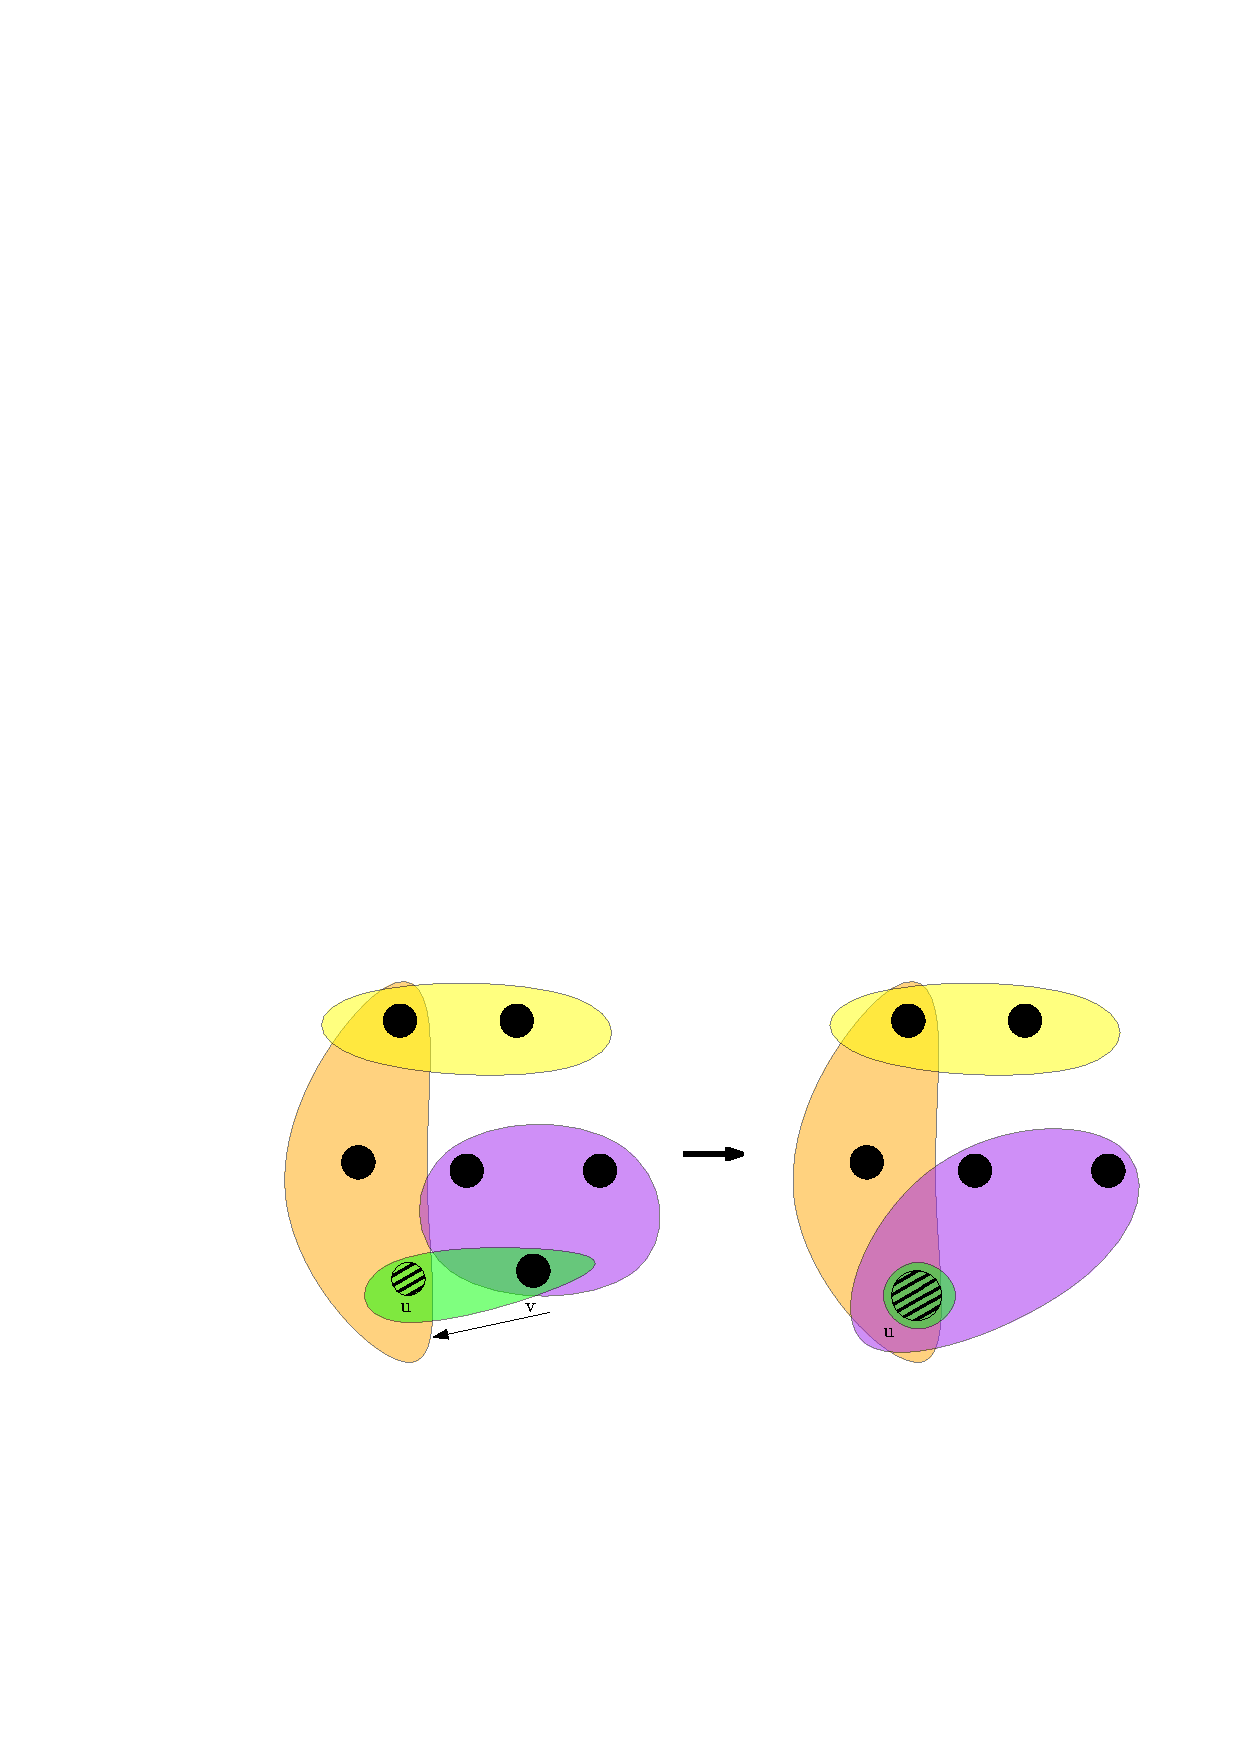
\includegraphics[width=.8\textwidth]{Ipe/Coarsening_Example.pdf}
  \caption{An example of a contraction. Note that the Hyperedges of the reduced node $v$ are rearranged to contain $u$.}\label{fig:coarsening_example}
    \vspace*{-.5cm}
\end{figure}


%Hypergraph := (H;V;E;C)
%Node contraction := 
%Node uncontraction := 
%Net :=
%cut :=
%onnectivity :=
%quality :=
%p%opulation :=
%individual :=
%solution := 
%mbalance:= 
\section{Related Work}
%A Hypergraph cannot be reduced to a graph with clique representation without skewing the cut metric \cite{ihler1993modeling}

There are several methods for partitioning Hypergraphs resulting from VLSI design and circuit partitioning. Cong and Smith \cite{cong1993parallel} provided a multilevel hypergraph bisectioning algorithm, using the netlist rather than the hypergraph. 

More powerful tools like PaToH \cite{catalyurek1999hypergraph} partition the hypergraph using the multilevel paradigm and try to improve solution quality by using v-cycle operations like hMetis\cite{karypis1999multilevel}. 

The hypergraph partitioner KaHyPar additionally improves on solution quality optimizing on the connectivity metric using k-way partitioning \cite{akhremtsev2017engineering} as well as cut using recursive bisection\cite{schlag2016k}.  
KaHyPar also uses a multilevel approach for partitioning \ref{fig:coarseningexample}. The original hypergraph $H$ is coarsened by repeatedly contracting nodes $u,v$ until either no more contractions are possible due to the size of the contracted nodes or that the minimum amount of nodes required to be in the coarsened Hypergraph $H_c$ has been reached. During each step of the coarsening only one pair of nodes $u, v$ is contracted. The contraction should preferably choose highly connected vertices, resulting in smaller and fewer hyperedges. Therefore the best contraction partner is determined for each vertex, counting the amount of shared hyperedges. There are some difficulties regarding validation of the calculated values after a contraction has been performed, resulting in different approaches regarding the coarsening step.
%TODO explain node selection for coarsening 
On $H_c$ a partitioning algorithm is chosen to generate an initial partitioning for the coarsened Hypergraph. Afterwards to contraction operations will be reversed and 
during each step of the uncoarsening phase local search algorithms are used to improve the current connectivity of $H$. The local search is using a variant of the Fiduccia-Mattheysis algorithm \cite{fiduccia1988linear}. 
\newline
\begin{figure}[H] 
    \vspace*{-.25cm}
  \centering
   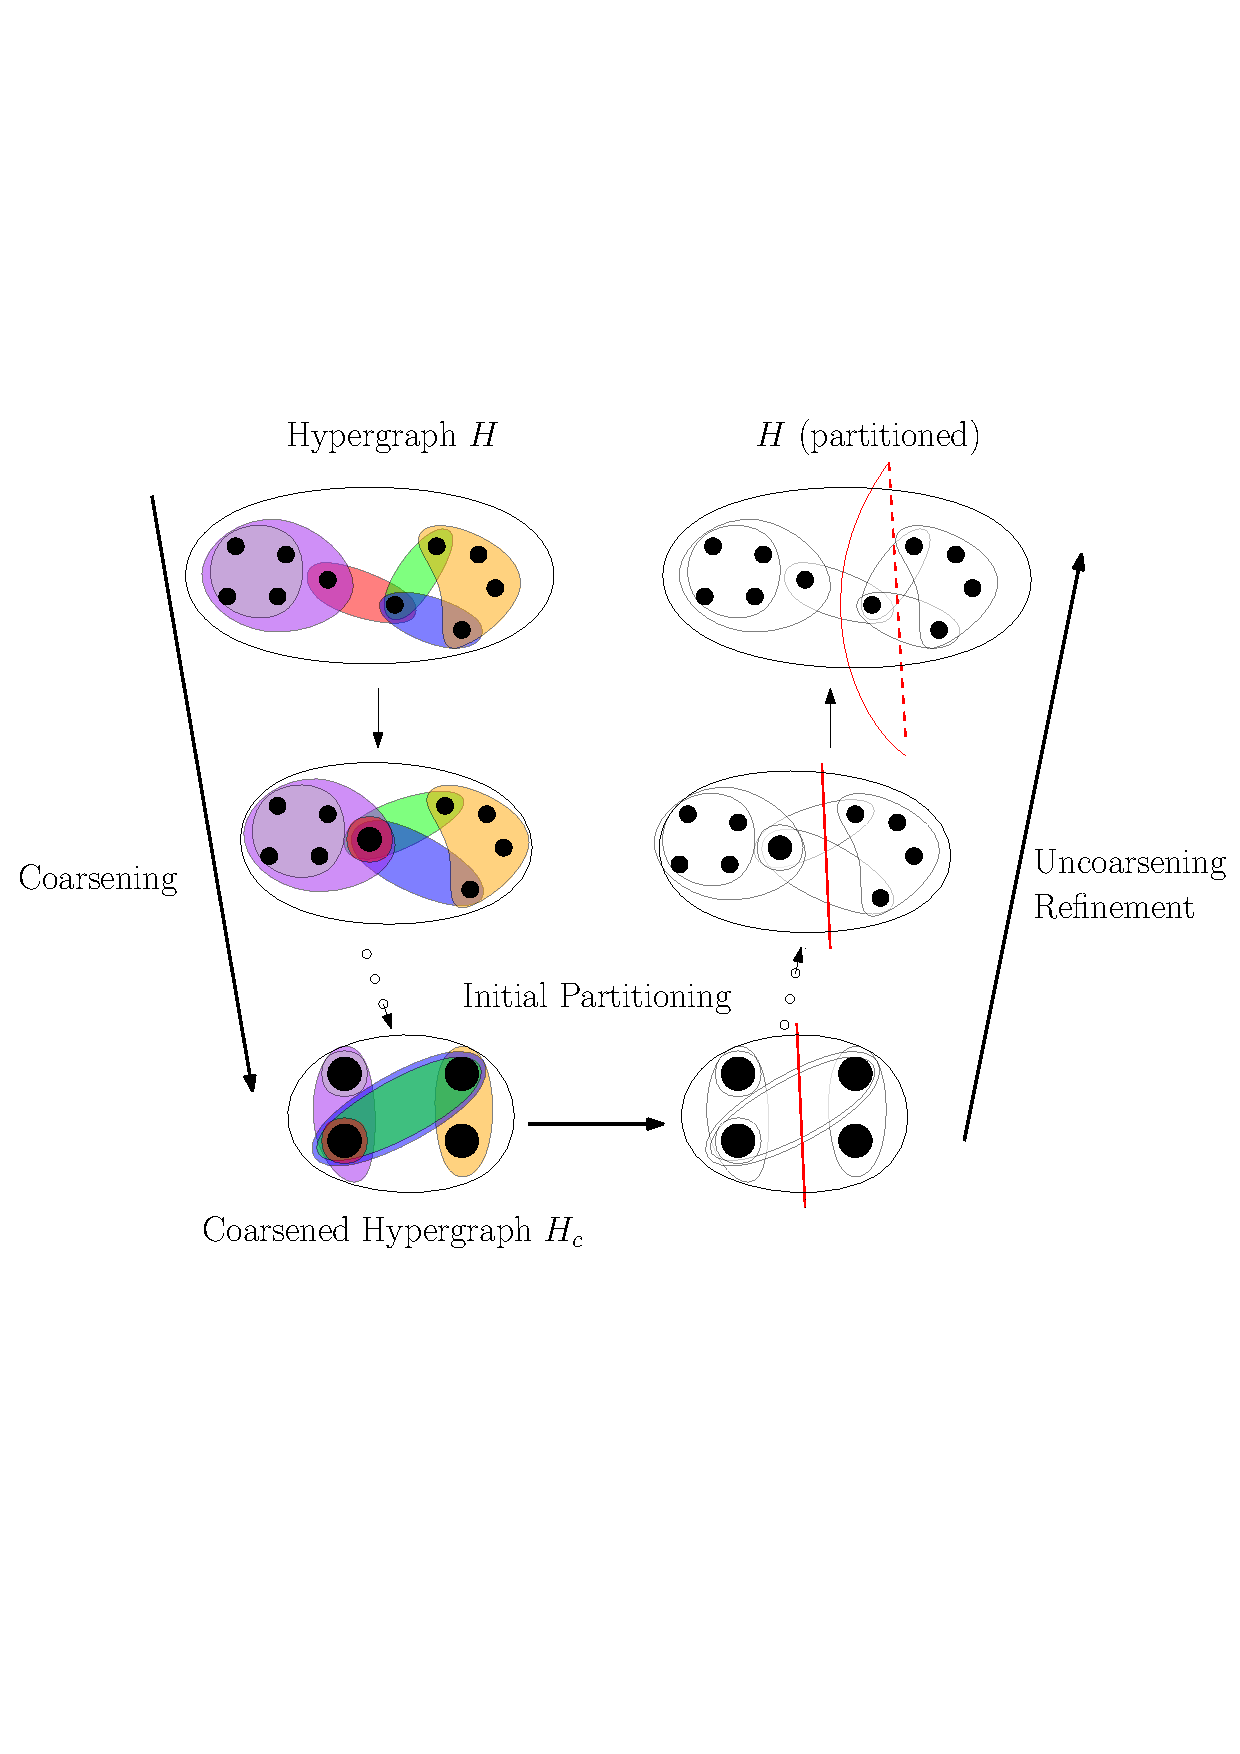
\includegraphics[width=.8\textwidth]{Ipe/Memetic_process.pdf}
  \caption{An example of an iteration. Coarsening, Initial Partitioning and Refinement}\label{fig:coarseningexample} %TODO u nicht gestrichelt; pünktchen
    %\vspace*{-.5cm}

\end{figure}
In 2017 Heuer and Schlag improved KaHyPar by analyzing and exploiting community structures in Hypergraphs \cite{heuer2017improving}, showing that KaHyPar-CA generates solutions of superior quality compared to other established hypergraph partitioners.


Saab and Rao \cite{saab1989evolution} present one of the first evolutionary approaches to hypergraph partitioning by iteratively performing vertex moves comparing the gain to a random threshold and processing the unique blocks in sort order. Hulin \cite{hulin1990circuit} presents a genetic algorithm maintaining multiple solutions using a two dimensional representation of circuits accounting for the gate level and atomic level , introducing a problem specific crossover operator as well as a mutation on either the gate or atomic level. A more high level memetic algorithm for the hypergraph partitioning problem was created by Bui and Moon \cite{bui1994fast}, in which solutions are preprocessed and optimized using the Fiduccia-Mattheyses \cite{fiduccia1988linear} local search algorithm as well as a new replacement strategy considering the solution quality as well as the similarity. 

Chan and Mazmudner\cite{chan1995systolic} provide an genetic algorithm for bipartitioning that assigns better solutions a higher chance to be selected for the crossover operation. The crossover operation splits both input partition at the same point combining the first split of the first partition and the second split of the second partition.
Areibi \cite{areibi2000integrated} gives another memetic algorithm in consideration of the k-way hypergraph partitioning problem using a variation of FM designed for k-way optimization \cite{sanchis1989multiple} local search as well as a 4-point crossover operation, which splits the input partitions at 4 points and alternates between the blocks.
\cite{kim2004hybrid} Kim et al. translate the lock gain local search \cite{kim2004lock} for graphs onto hypergraphs and use solution quality and hamming distance as a more potent replacement strategy as well as roulette selection to determine the solutions used in the crossover.
 Sait, El-Maleh and Al-Ajabi \cite{sait2006evolutionary} compare the metaheuristics tabu search, simulated annealing and genetic algorithms for k-way hypergraph partitioning.
Armstrong, Grewal, Darlington and Areibi\cite{armstrong2010investigation} are analyzing the quality and run time performance of a parallel memetic algorithms using local search for two iterations, until no further improvement can be made, and a combination of both. All referenced works that use a crossover operator do so by splitting the input partitions and selecting alternating block fragments.



Sanders and Schulz created an evolutionary framework \cite{sanders2012distributed} for the existing graph partitioner KaFFPa, \cite{holtgrewe2010engineering} introducing different combination and mutation operations for graph partitioning. Their approach uses the mulitlevel paradigm in combination with evolutionary operations to gain improvements in the solution quality. This is the framework KaHyPar-E is trying to create for hypergraphs.
%KaHyPar
%KaHiP 
%edge-frequency
%%%%%%%%%%%%%%%%%%%%%%%%%%%%%%%%%%%%%%%%%%%%%%%%%%%%%%%%%%%%%%%%%%%%%%
%TODO only one individual is generated per iteration
%TODO explain evolutionary algorithms, or at least show that this is one
\chapter{KaHyPar-E}
In this chapter we first outline the general procedure of an evolutionary algorithm. Then we transfer the hypergraph partitioning problem onto an evolutionary framework supporting the 
theoretical foundation. Then we introduce operators for combination and mutation as well as strategies for selection and replacement.
\section{Overview}
Evolutionary algorithms are inspired by the theory of evolution. Much like the biological counterpart they attempt to simulate 
an enclosed space where several actors, or individuals, try to compete for survival and reproduction in an isolated setting over the timespan of multiple generations.
The evolution theory states that individuals having more helpful traits like special beaks to assist in aquiring food are more likely to survive longer and 
thus more likely to pass these helpful traits onto the next generation. Addiditionally some traits occur randomly through chaning the genetic information with no direction of helpfulness regarding suruvival. These are called mutations and are even present in humans, like the sickle-cell desease or the ability to consume lactose. In the evolution theory mutations 
are usually a factor that introduces previously nonexistent traits, which would have been unable to recreate using reproduction alone. Repeating the cycle of survival and reproduction the mutations that are helpful will more likely be passed on and established. Based on this principle evolutionary algorithms are essentially converting the process described above onto a mathematical problem. Therefore some initial solutions are generated and then the same steps are repeated until a stopping criterion has been met.
Evolutionary algorithms are usually repeating 4 steps trying to simulate evolution. First some individuals have to be chosen for recombination. Then the chosen individuals have to be combined with each other generating offspring. As third step mutations are performed on some individuals and as fourth step the individuals surviving the iteration(generation) are selected by a corresponding metric, also called fitness. For hypergraph partitioning we consider a partition as an individual and the fitness of said individual is the cut or connectivity metric. We alternate the evolutionary scheme a bit in a sense that we perform combination or mutation exclusively during an iteration and additionally only generate one new solution during said iteration and then replace an existing individual with the new offspring. 

\section{Population}

The algorithm will produce multiple individuals, which are inserted and removed from the population. At any given time only a finite amount of
individuals are $alive$ which is the maximum population size. Further individuals have to compete for a place in the population. 
The population size is an important parameter, as a small value limits the solution scope and a high value limits convergence \cite{chen2012large}.
We use KaHyPar to fill the initial population. This means that unlike most evolutionary algorithms we use high quality solutions instead of random solutions as initial population.
In order to select a proper population size for the runtime we attempt to allocate a fair amount of time towards the creation of the initial population. 
By measuring the duration of one iteration $t_1$ and comparing it to the total runtime ${t_{total}}$ we can estimate the amount of iterations $\frac{t_{total}}{t_1}$. Since hypergraph instances
vary greatly in time required to partition, using a fixed population size will most likely be unfitting for most instances. As a solution we try to use a fixed amount of time for generating 
individuals for the initial population by evaluating the value calculated above and spend approximately 15\% of the alloted time towards creating the initial population and the population size is determined by $0.15*\frac{t_{total}}{t_1}$.
However we introduce lower and upper bounds for the population size to ensure a proper size for evolutionary operators and convergence. That being said the population size has to be at least 3 and 50 at most.
\section{Diversity}
%By measuring the difference between two individuals we can gain some knowledge over their internal structure and similarities.
Diversity represents the distance of two solutions in the solution space. Maintaining diversity is highly recommended\cite{back1996evolutionary}.
A high diversity in the population is representing a high coverage of the solution space and 
thus enables the evolutionary operations to traverse a greater portion of solutions. 
Vertices are not directly influencing either metric and therefore not a good option to measure diversity. Instead we analyze the cut edges of the two solutions 
on differences. By counting the edges which are in the cut in exclusively one of the two solutions we gain a numerical value representing the difference. This model is easily applicable for 
graphs but falls short on hypergraphs. \ref{fig:diversity} Instead we count the differences of the amount of blocks for each edge. This is a more natural representation for the connectivity metric as cut edges might easily extend to additional blocks. If the diversity in the population is low it means that the individuals have converged.

\begin{figure}[H] 

    \vspace*{-.25cm}
  \begin{center}
   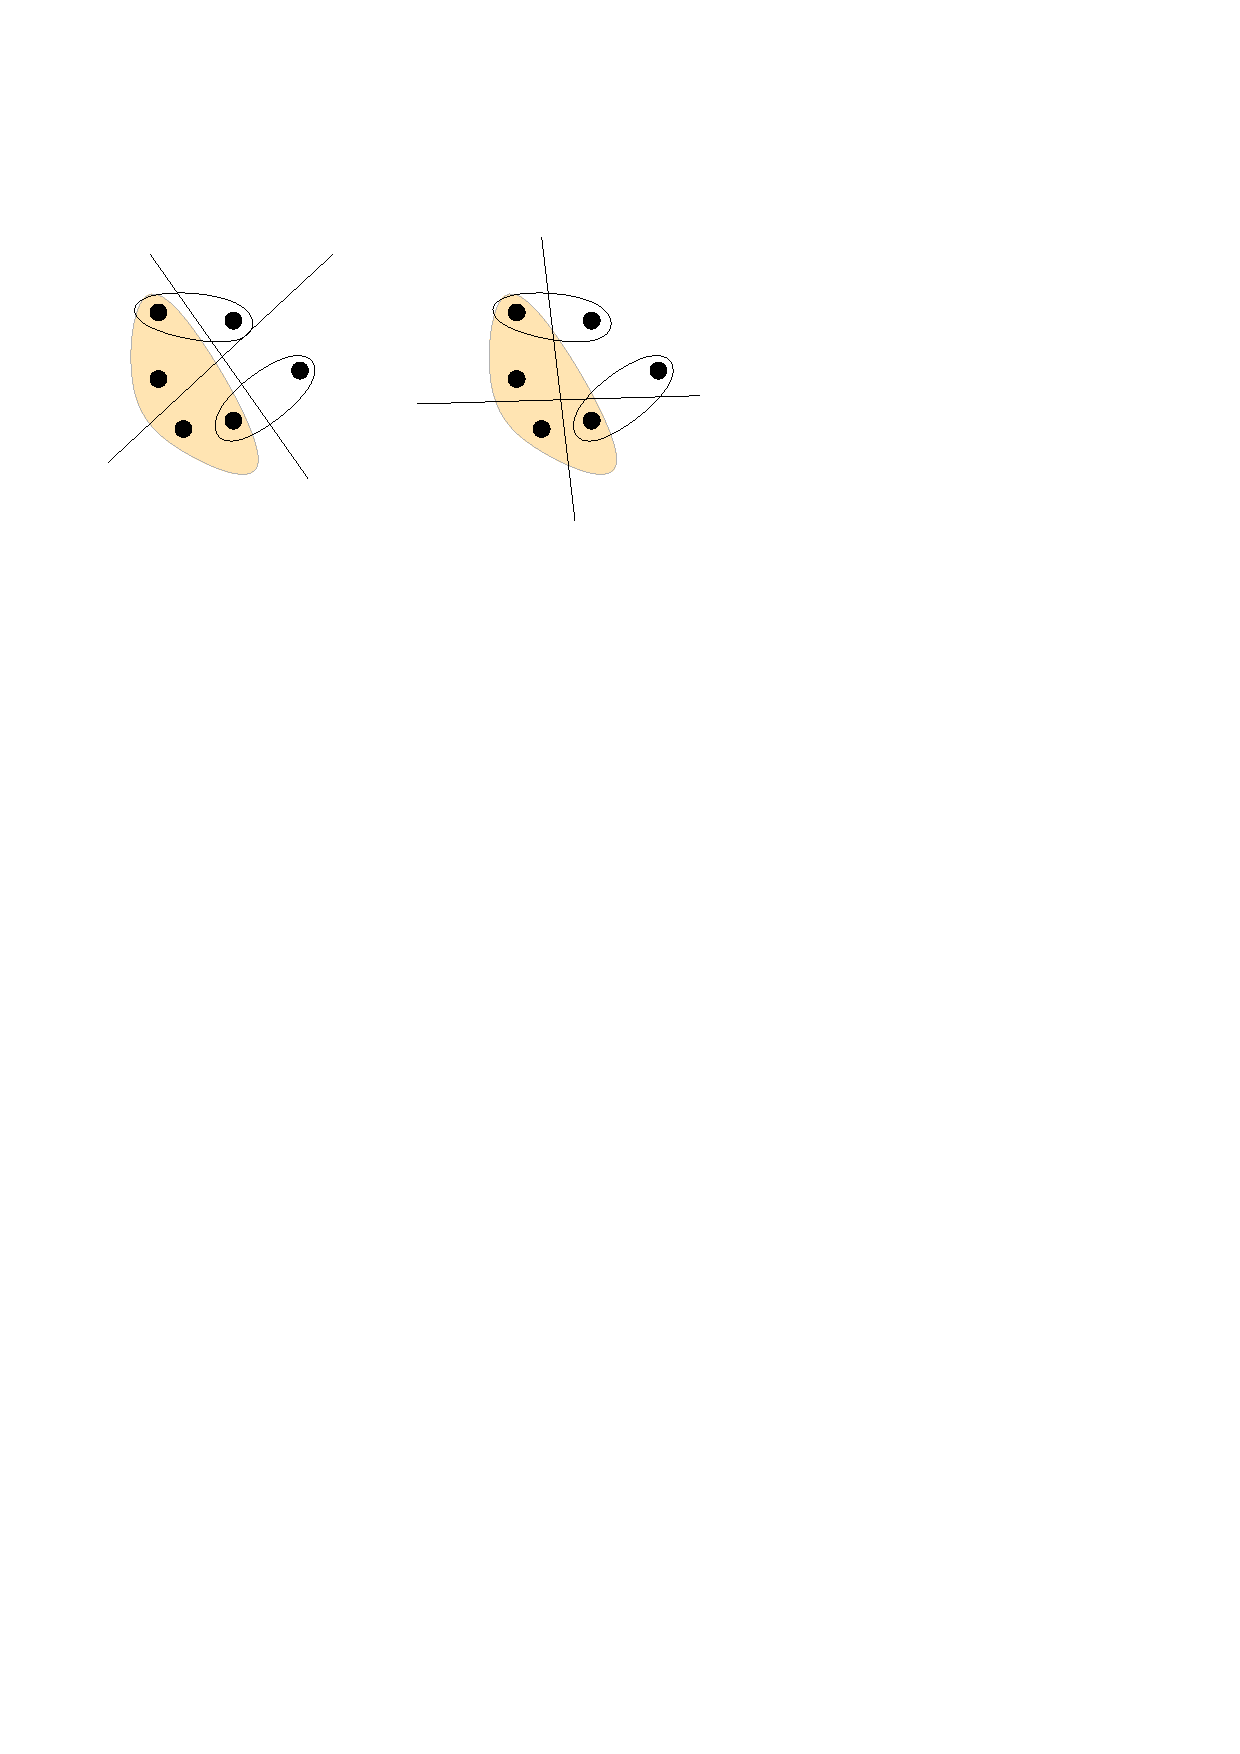
\includegraphics[width=.8\textwidth]{Ipe/connexample.pdf}
  \caption{Two different partitions of the same hypergraph}\label{fig:img.png} 
  \label{fig:diversity}
    %\vspace*{-.5cm}
  \end{center}
  In this figure you can see two different partitions of the same example hypergraph. Since all edges are a cut edge the simple difference is 0. However the partitions are not to be considered equal since the highlighted edge has 
  a different amount of blocks in the two partitions. By using the strong difference this error can be avoided. 
\end{figure}

\section{Selection Strategies}
For an evolutionary algorithm we attempt to generate new, improved solutions by using existing solutions. A logical conclusion is that good individuals probably will generate solutions
close to the original individual and as result similarly good. We select our individuals using tournament selection \cite{blickle1996comparison}, meaning that the individuals are competing for their chance of recombination by their fitness. In a long term perspective this ensures that good individuals get a more frequent chance of reproduction as stated by the evolutionary theory.  By first selecting two random individuals and using the one with the better solution quality we can extract one individual $I_1$ while better solutions are more likely to be used by the algorithm. For operators requiring two seperate Individuals we can simply redo this step to gain a new individual $I_2$. In the unlikely case that the two selected individuals are the same we instead use the worse individual from the second tournament selection.
\section{Combine operations}
Combine operations generate a new individual by using two or more individuals as input. The premise is that the good characteristics in regard to the fitness should be exploited for the 
generation of new solutions. The basic combine operator C1 uses tournament selection to determine the parent partitions. The edge frequency multicombine operator C2 strictly uses the best
partitions in the population. Both operators use the replacement strategy introduced in \ref{sec:replacement} to insert the newly generated individuals.
\subsection{Basic Combine (C1)}
\label{sec:basiccombine}
The basic combine uses two parent partitions $P_1$ $P_2$ in order to create a child individual $C$. This is achieved by only allowing contractions of nodes $u, v$ when these nodes are not placed in different partitions in either parent. We only perform contractions which do not harm the quality of either $P_1$ or $P_2$, as none of the contractions would cause a node to switch blocks in either partition, thus maintaining their quality during coarsening. 
Afterwards we do not perform an initial partitioning, instead we consider the coarsened hypergraph $H_c$ and see which of the parents gives the better objective on $H_c$.
The important part to note is that this operation is different than a v-cycle, since the coarsening condition is more strict due to the consideration of both parents partitions. The uncoarsening and application of local search algorithms which do not worsen solution quality in combination with using the better partition of the two parents ensures that the child solution is at least as good as the best parent solution. \label{qualityassurance} The basic combine is benefitting from highly diverse parent partitions since it causes more strict limitations during the coarsening, which means more information passed onto the child individual. In terms of solution scope the operation is highly convergent due to the quality assurance and strong limitation during the coarsening. 


\subsection{Edge Frequency Multicombine (C2)}
\label{sec:edgefrequency}
We also introduce a multi-combine operator, capable of combining multiple individuals $I_1.. I_n, n \le |P|$ into a new child individual. By analyzing whether an edge $\textbf{e}$ is a cut edge in $I_1 ..I_n$ we can calculate the edge frequency \cite{wichlund1998multilevel} of $\textbf{e}$ by $f(\textbf{e}) := \sum_{i=1}^n cut(\textbf{e},I_i)$. We use the best $n = \sqrt{|P|}$ individuals from $P$ for determining edge frequency as a standard parameter \cite{delling2011graph}. Considering the best solutions edges with a high frequency are more likely to be cut edges in equally good solutions. Therefore we penalize contractions of nodes incident to a high frequency edge during the multilevel partition approach by using this formula
\begin{center}
$gain(u,v) = \dfrac{e^{-\gamma*f(\textbf{e})}}{(w(u)w(v))^{1.2}}$ 
\end{center}





to disincentivize early contractions of nodes in edges of high probability. w(u), w(v) are the weights of the nodes and $\gamma$ is a dampening parameter. Please note that the simple e in the formula is not a reference to the edge but rather to the eulers number. When using this gain value during the coarsening phase of KaHyPar, contractions of high frequent edges are losing up to 40\% in gain calculation using $\gamma = 0.5$ which is the default parameter from \cite{wichlund1998multilevel}.
 he only step that differentiates this operator from a regular iteration using KaHyPar is that the rating function during the coarsening is adapted by the updated gain formula above. As such a new initial partitioning as well as uncoarsening and refinement are required. Since this operation is generating a new initial partitioning there is no quality assurance opposed to C1.
%\subsection{Basic Combine + Edge Frequency Information}
\section{Mutation operations}
The v-cycle mutations introduced in this chapter are performed on randomly chosen individuals instead of tournament selection. They require one input individual. Stable Net mutation however is using multiple individuals, similar to C1. The main objective of mutations is to create more diverse solutions and to improve current solutions to avoid population convergence towards a local optimum.
\subsection{V-Cycle (M1)}
A v-cycle is an iteration in the regular KaHyPar procedure with the difference that $H$ is already partitioned. During the coarsening nodes $u,v$ may only be contracted if $part(u) = part(v)$. Since the hypergraph is already partitioned there is no need for initial partitioning. The main benefit comes from the refinement during the uncoarsening. This operation takes one individual $I$ and the result is a similar individual $I_new$ which has been improved on during the refinement. Due to the fact that neither refinement nor coarsening worsen the quality of the solution $I_new$ will have a quality at least equal to $I$. This is a weak mutation and the difference of $I$ and $I_new$ are small. This operation will also cause convergence, as multiple applications of a vcycle will eventually no longer be able to generate improvement and are unable to escape the local optima due to the fact that worse solutions can not be generated. This operation is also used in KaHyPar-CA + vcycle as the strongest configuration of KaHyPar-CA. However the number of v-cycles performed during one evolutionary iteration is 1, whereas the number of v-cycles performed during one iteration of KaHyPar-CA + vcycle is arbitrarily high to only stop when no further improvements have been found.
\subsection{VCycle + New Initial Partitioning (M2)}
Similar to a v-cycle we can coarsen $H$ with a partition limiting the coarsening, but instead of immediately starting the refinement we drop the partition and perform a new initial partitioning on the coarsened Hypergraph. This operation pertubes the original more strongly because the vertices are no longer forced to keep their assigned block. Since the partition is
dropped the algorithm used to generate a new partition might produce a worse solution as before. Therefore this operator can create worse solutions and as a result the operator is capable of introducing diversity regardless of current convergence in the population. 
\subsection{Stable Nets (M2)}
Edge frequeny is the operator where edges of high probability of being in the cut are penalized because these edges are most likely being in the cut. Stable net \cite{lim1997large} removal attempts to broaden the solution scope by forcefully removing high frequency edges out of the cut, opposing the goal of edge frequency. Again the $\sqrt{|P|}$ best individuals are analyzed, regarding edges most frequent in these solutions. We consider an egde stable if it is in the cut in at least 80\% of the inspected individuals. These edges are then attempted to be forced into the block with the smallest amount of nodes in order to keep the balance criterion met. Forcefully moved nodes may not be reassigned through another stable net. These solutions have most likely siginficantly worse quality. Due to the nature of our selection strategy these solutions are very unlikely to be used in any combine operator. In order to keep these solutions competitive we also perform a vcycle after removing the stable nets. This operator is intended to create individuals significantly different. 
\section{Replacement Strategies}
\label{sec:replacement}
Regardless of the operator, the generated individual has to be inserted into the population in order to be used in upcoming iterations. We elitist reproduction approach generating only one new individual each iteration. And since the only way to remove an individual from the population is by insertion of the new individual also the driving factor of selection. 
The naive approach is to remove the worst element from the population and insert the individual in its place, with the intention to ensure a vast majority of the best generated solutions.
The consequence is that the population is rapidly converging towards a local optima and only covering a small amount of the solution space. Another approach is to replace the element used in the operator. This strategy was originally used for mutations, as the theory behind evolutionary algorithms is to pertubate an existing solution. But this approach completely neglects fitness, the main reason to use selection as a tool. 
We use a different strategy maintaining the competitive pressure of the selection whilst also avoiding premature convergence. Similar to the naive approach we consider the fitness of the newly generated individual to replace an individual with worse quality. However we do not replace the worst existing element, instead we replace the most similar element with a worse quality using diversity as measurement for similarity. This leads to a similar competititveness in selection, thus driving the population towards convergence. However it ensures a more diverse population 
which boosts the combine operator effectiveness and avoids rapid convergence. In fact when considering the population slots rather than the single individual it results in the multiple small convergence lines towards several different local optima while improvements can be made and a convergence towards the best optimum as soon as all slots found a local optimum. 

\begin{figure}[H] 

    \vspace*{-.25cm}
  \begin{center}
   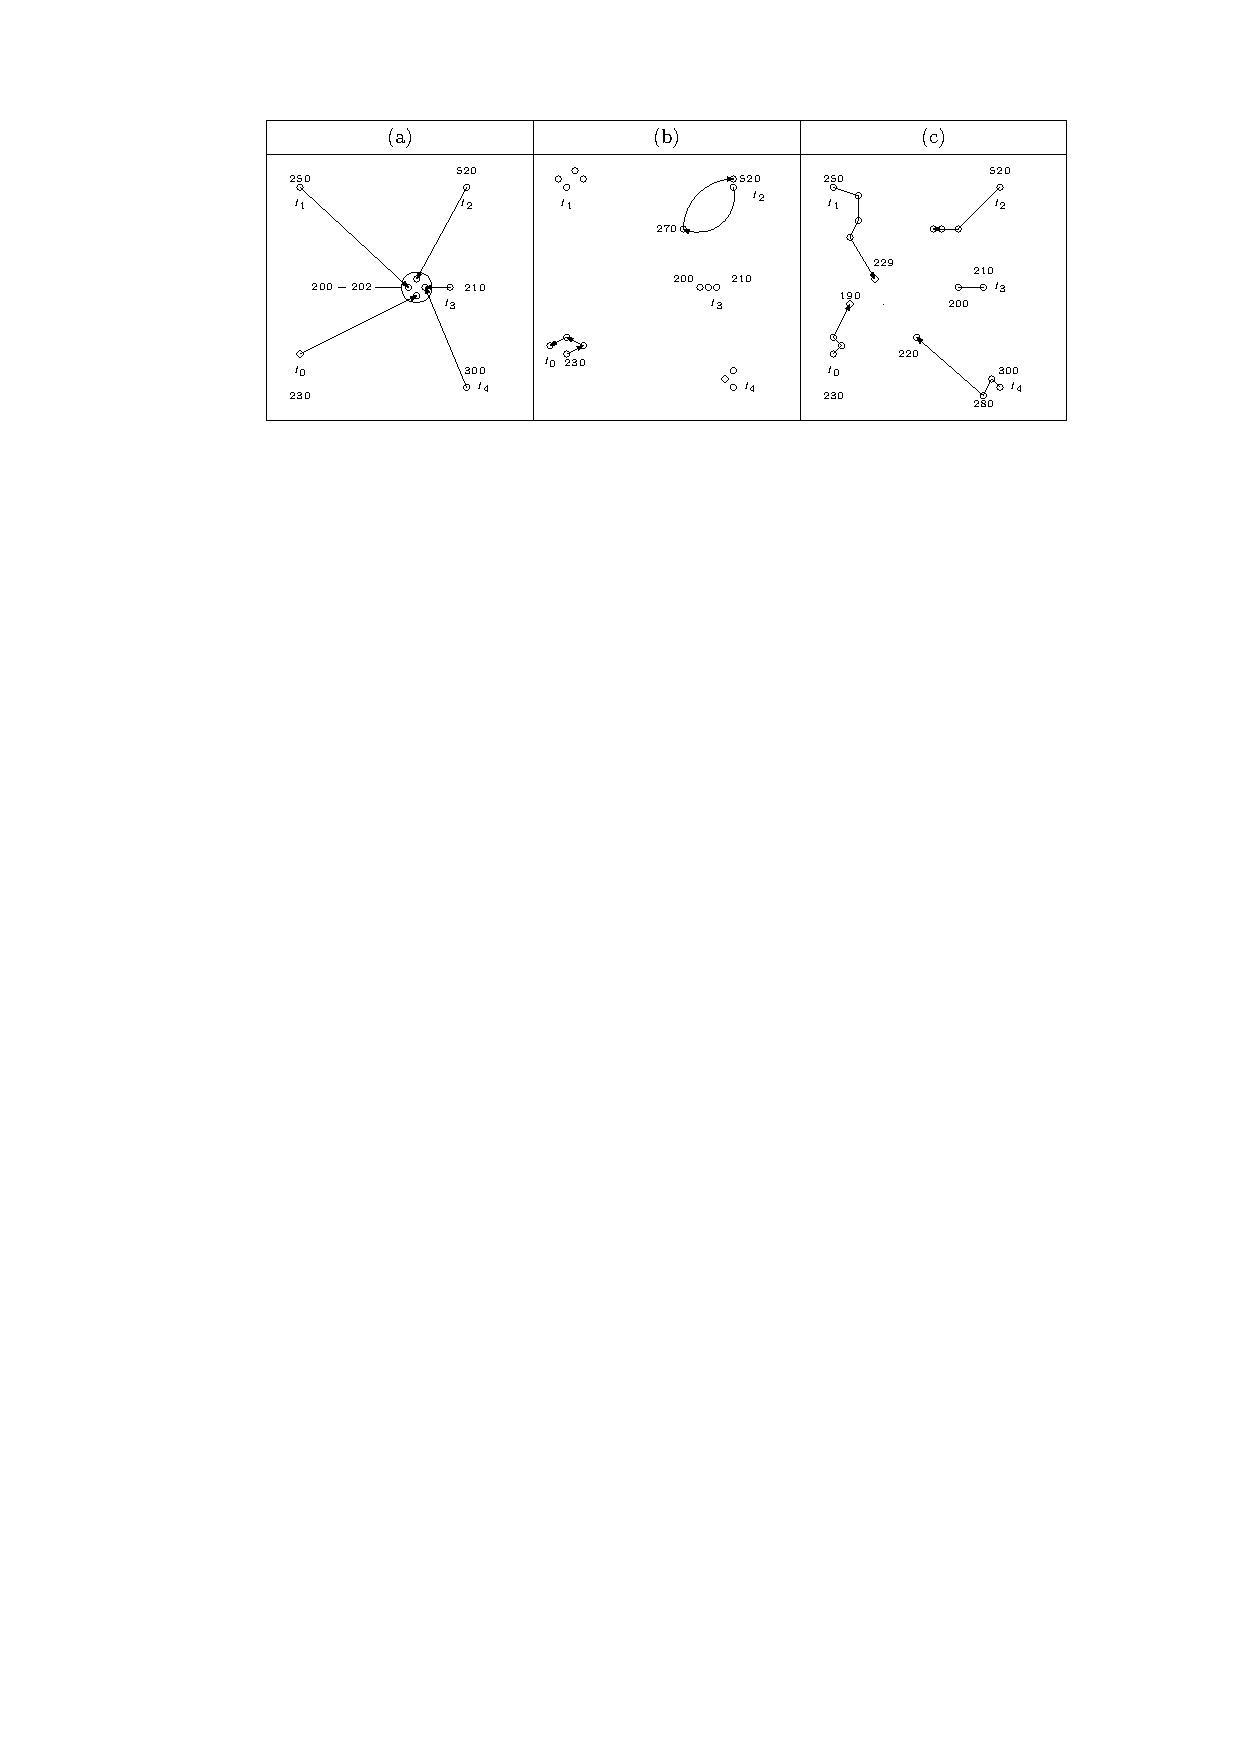
\includegraphics[width=.8\textwidth]{Ipe/diverse_example.pdf}
  \caption{Visual representation of different replacement strategies (a) replacing the worst element, (b) replacing the most similar element \& (c) replacing similar/worse}\label{fig:img.png} 
  \label{fig:diverse_graphic}
    %\vspace*{-.5cm}
  \end{center}
  In \ref{fig:diverse_graphic} the diversity of the elements is displayed as distance in the 2D plane. The arrows represent whenever an individual is replaced. In (a) a fast convergence towards the local optimum near $I_3$ is happening. Due to the premature convergence and strictness of the replacement strategy there it is highly unlikely that any solution will ever leave this local optimum. In (b) each individual solution is replaced more thoroughly, but good solutions are found at random and may be discarded at any moment. In (c) each of the five slots in the population is slowly converging towards its own respective local optimum, but eventually the best local optimum forces convergence. Note that this graphic is only displaying replacements. The individuals involved in creating these solutions are not linked to the replacement. i.e. $I_3$ at 210 might have been replaced with a solution of quality 200, but the elements creating the solution have been $I_1$ and $I_2$.
\end{figure}

%.....
%%%%%%%%%%%%%%%%%%%%%%%%%%%%%%%%%%%%%%%%%%%%%%%%%%%%%%%%%%%%%%%%%%%%%%
\chapter{Experimental Evaluation}

%#<<test, fig=TRUE, echo=FALSE>>=
%#x = rnorm(100)
%#y = rnorm(100)
%#plot(x,y)
%#@
%Vcycle Mutations
All following plots are using KaHyPar for generating an initial population and perform some of the mentioned operators.
%base with nonevo and random combines












\section{Implementation}
\section{Experimental Setup}
\subsection{Environment}
We evaluate our algorithm on two Hypergraph sets. One time for different $k = \{2,4,8,16,32,64,128\}$ and 174 Hypergraph Instances, repeating
each run 5 times with different seeds and a algorithm runtime of 8 hours. This is referenced as benchmark subset. The other evaluation is a
selection of 25 Hypergraphs using only one $k = 32$ and a runtime of 2 hours. This is referenced as tuning subset. 
As such our datasets contain multiple tuples of $(H, k, s, t, \lambda)$ where $H$ is the instance, $s$ the seed, $t$ the required time and $\lambda$ the solution quality. An Instance $I$ is the subset of $(H, k, s, t, \lambda)$ where $H$ and $k$ are fixed.
The main interest is the best solution over time compared to other partitioning algorithms. Unfortunately most graphs vary drastically in solution quality and time required to perform one iteration. We solve the time differences by not using the measured time, but rather the normalized time. 
In order to do so we choose one of the partitioning algorithms $p$ as baseline and determine the average duration $t_I$ of an iteration for each $I$. Afterwards for each $I$ the normalized time $t_n$ is calculated by $t_n = \frac{t}{t_I}$. We then generate a list for each instance containing $(s, t_n, \lambda)$ sorted by $t_n$. Now we generate the averaged improvements for $I$. For each seed $s$ a value $a_s$ is reserved and the list is read in. When $(s, t_n, \lambda)$ is better than the reserved value for $s$ the average over all $a_s$ 
is the new value appended to the averaged improvements with($(avg(a), t_n)$. Similarly we now reserve a value $a_I$ for each Instance of averaged improvements and calculate a new list of general improvements by calculating the geometric mean over all $a_I$. 

\begin{figure}[H] 
    
  \begin{center}
   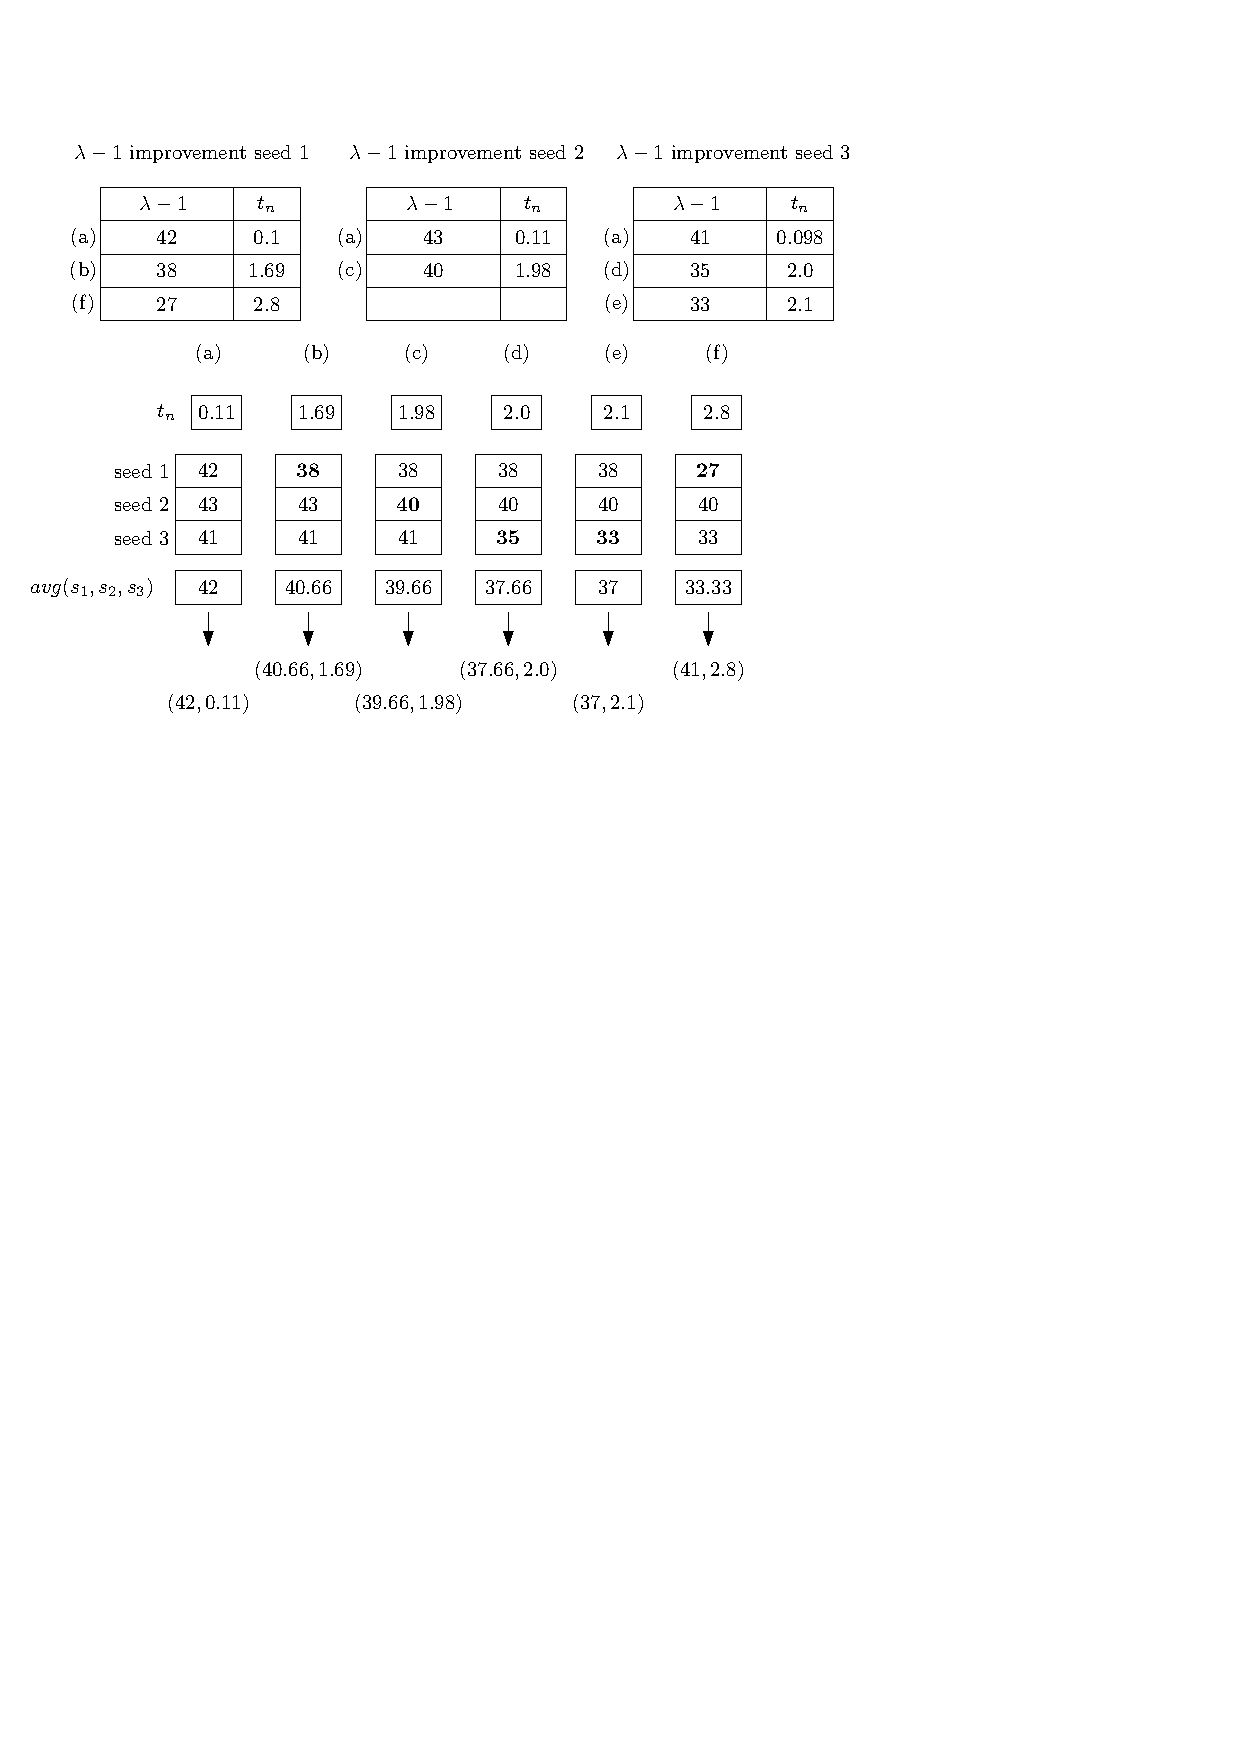
\includegraphics[width=.9\textwidth]{Ipe/seed_averaging_example.pdf}
  \caption{An example for averaging the seeds of an Instance $I$}\label{fig:img.png} %TODO u nicht gestrichelt; pünktchen
  \end{center}
    The solution improvements of the different seeds are run through by ascending normalized time $t_n$ (a)-(f). Then a pair of solution quality and current time is appended to the result every time an improvement is found (b)-(f). The only exception is (a) since there are no existing values to replace. In this case the first values of all seeds are used and the maximum normalized time is used for the first pair.
\end{figure}

\subsection{Tuning Parameters}
The parameter spectrum of the evolutionary algorithm is rather voluminous. Beginning with the different chances of the combine and mutation operations to be chosen. As such we first evaluate the operations themselves before tuning the respective chances. The first chance is the amount of mutations performed in contrast to combinations. As such the best value for mutation chance using new initial partitioning, the most powerful mutation operation results in a value of 40\% to 50\% for mutation chance. This is drastically diverging from the chance used in evolutionary graph partitioning which is around 10\%. \cite{sanders2012distributed}
\begin{figure}[H]
\caption{New initial partitioning mutation chance}
\begin{center}
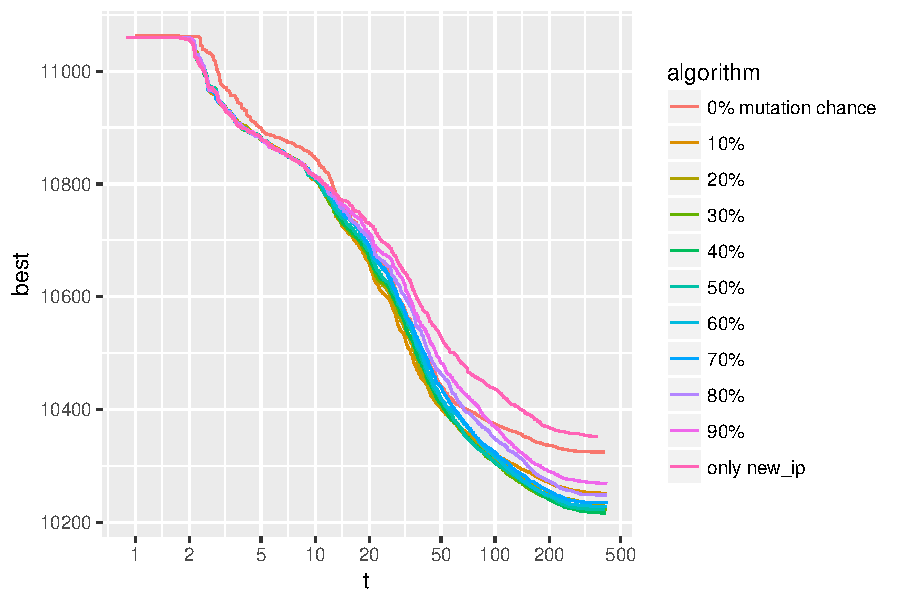
\includegraphics{bachelorarbeit-newipmutationchance}
\end{center}
In this plot the different mutation chances are represented. The percentages represent the chance of performing a new initial partitioning vcycle. If not performing a new initial partitioning a basic combine is performed. It is visible that choosing either 0\% mutation chance or 100\% mutation chance are both not viable for generating good solutions. A combination of both operators is increasing solution quality. As seen in this experiment a mutation chance of 40\% for new initial partitioning is generating the best solution. This experiment was performed on the tuning subset to generate values for the run on the benchmark subset.
\end{figure}

Additionally for tuning the chances of selecting a mutation the chance of performing an edge frequency combine can be tuned as well. Similarly to mutation operations it is quite visible that 

\begin{figure}[H]
\caption{Edge frequency chance}
\begin{center}
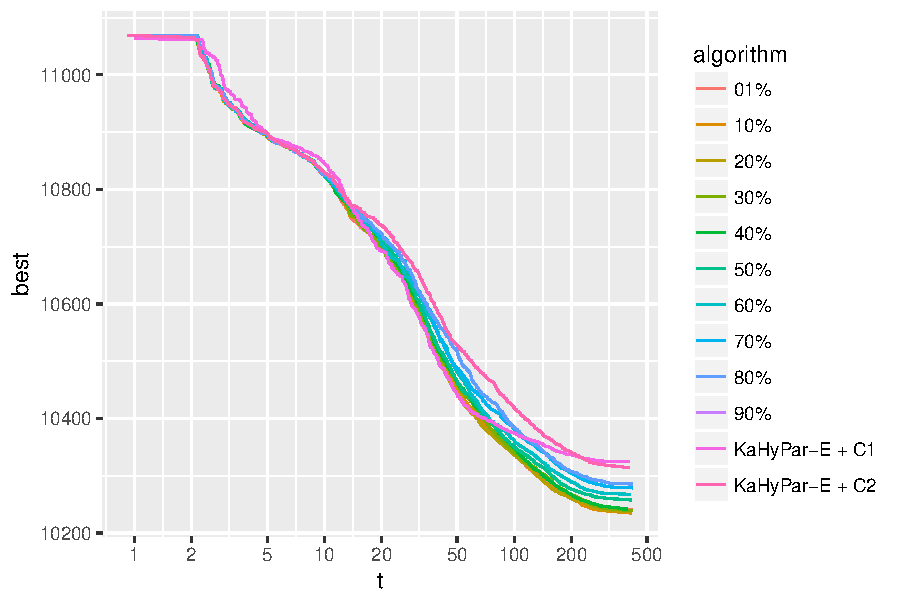
\includegraphics{bachelorarbeit-edgefrequencytuning}
\end{center}
In this plot the chances of performing an edge frequency instead of a basic combine are displayed. Clearly recognizable is that a proper application of both operators will lead to improvements. The optimal values are in a range from 20\% to 50\%, however similar to the mutation chance tuning no significant difference can be observed between the tuned values.  
\end{figure}
\subsection{Instances}

\section{Your Experiment Headline}

%%%%%%%%%%%%%%%%%%%%%%%%%%%%%%%%%%%%%%%%%%%%%%%%
%%%%%%%%%%%%%  EVALUATION KAHYPARE BEGIN %%%%%%%
%%%%%%%%%%%%%%%%%%%%%%%%%%%%%%%%%%%%%%%%%%%%%%%%
\begin{figure}[H]
\caption{Comparing KaHyParE to KaHyPar}
\begin{center}
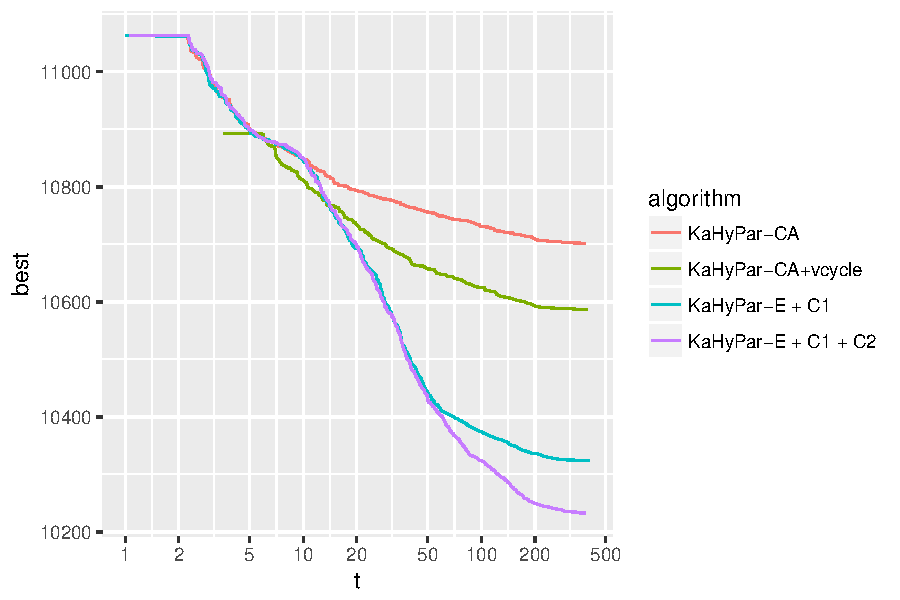
\includegraphics{bachelorarbeit-basiccomparation}
\end{center}

\end{figure}
In this plot we evaluate the results of KaHyParE using only basic combines as evolutionary operation against repeated repetitions of KaHyPar-CA and KaHyPar-CA + vcycles which is the strongest configuration for KaHyPar-CA. This evaluation is performed on the tuning subset. The plot lines of KaHyPar-CA, KaHyParE + C1 and KaHyParE + C1 + C2 are nearly identical up to the time point of 10 $t_n$ normalized time. This is due to the fact that KaHyParE is using KaHyPar-CA to generate the initial population. The variations are caused by hardware limitations causing minor fluctuation in the time for performing an iteration and thus slight variations in the normalized time. However the values generated are the same since KaHyPar-CA is configured with the same seed during each of those experiments. KaHyPar-CA + vycles is not sharing the same starting curve. Since v-cycles are time consuming the algorithm steps of KaHyPar-CA + vcycles are slower than the steps of KaHyPar-CA, resulting in an offset of the starting point for the plot line. As expected KaHyPar-CA + vcycles produces better solutions than KaHyPar-CA, which also extends to repeated repetitions. Both variations of KaHyParE gain a significant amount of improvement after generating the initial population. This is due to the combine schemes being able to exploit structural improvements by comparing different partitions as described in \ref{sec:basiccombine} and continually improving the solution quality by the assurance of nondecreasing solution quality \ref{qualityassurance}. However this operation is eventually converging into a local optima since all individuals are going to be replaced with the best solution in relatively close proximity due to the replacement strategy and neither replacement strategy nor operator are capable to decrease the solution quality of a given individual. the multicombine operation C2 however is not restricted to this assurance. This operator is profiting from a stable population in a sense that the best solutions in the population are most likely good solutions. This is visible in the plot since KaHyParE + C1 + C2 is not drastically different from KaHyParE + C1 while the basic combine is still effective but allows for an improvement of solution quality whereas KaHyParE + C1 is plateauing. Comparing KaHyPar-E + C1 against KaHyPar-CA + vcycles using the Wilcoxon-Pratt Test generates a $Z$-Value of 4.37 indicating that KaHyPar-E + C1 is computing better solutions with an error margin of 0.001\%.
%%%%%%%%%%%%%%%%%%%%%%%%%%%%%%%%%%%%%%%%%%%%%%%%
%%%%%%%%%%%%%  EVALUATION KAHYPARE END %%%%%%%
%%%%%%%%%%%%%%%%%%%%%%%%%%%%%%%%%%%%%%%%%%%%%%%%

\begin{figure}[H]
\caption{Different Mutation Operations}
\begin{center}
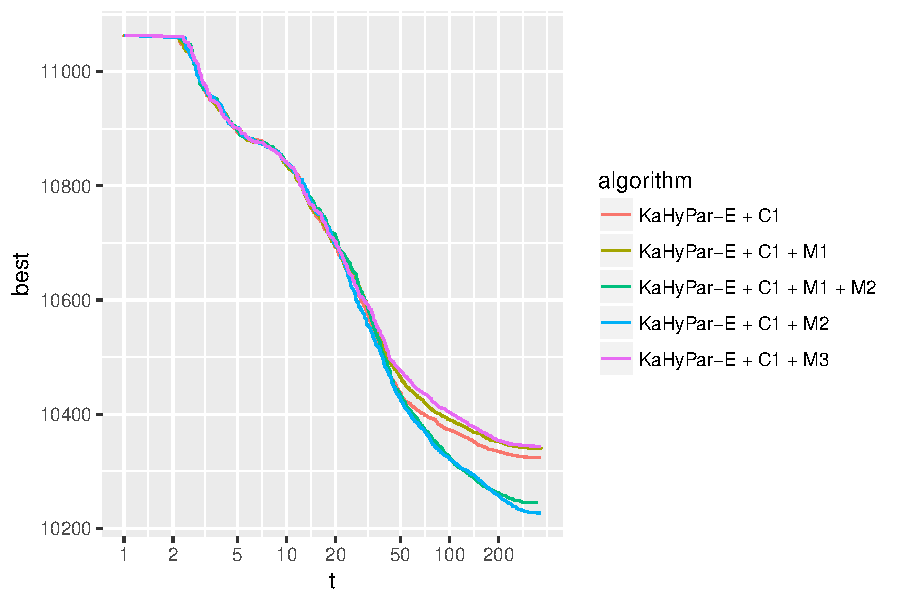
\includegraphics{bachelorarbeit-differentoperatos}
\end{center}
In this figure the effectiveness of the different mutation operators are evaluated. Each data set was created using a 50\% chance of C1 and a 50\% chance of the respective mutation operations. In the specific case M1 + M2 the mutation operation performed was selected uniformly at random. This evaluation was performed on the tuning subset. Adding simple v-cycles M1 to the already existing combine operator is in fact performing worse. This is due to the fact that v-cycles share the same quality assurance as C1 and are thus unable to create worse solutions which are necessary to broaden the solution scope of the population. Individuals that have been optimized during the execution of the algorithm also often have been improved by v-cycles or already have a good enough quality so that v-cycles cannot find improvements. In conclusion this means that v-cycles alone are unable to prevent premature convergence. In contrast using v-cycles with new initial partitioning M2 or a combination of both mutation operators will generate better solutions. Since M2 is not limited by the quality assurance of C1 and M1, worse solutions can be created and the solution scope can be explored more effectively. Stable net detection M3 is generating worse solutions or using up more time to generate individuals and therefore dropped from the algorithm. Interestingly when considering how often the different mutation operations have been able to generate a new best solution M3 has only been able to do so for 2 instances out of 25 whereas any combination of M1 and M2 have created a new best solution in all 25 instances. This suggests that M3 is an operation depending on the hypergraph structure and not easily applicable to a generic hypergraph. Due to the replacement strategy newly generated solutions are only considered for insertion if the solution quality is better than the worst individual in the population and will lead to convergence regardless of which mutation operators are applied. 
\end{figure}








%Cross combines
\begin{figure}
\caption{cross combines are bad}
\begin{center}
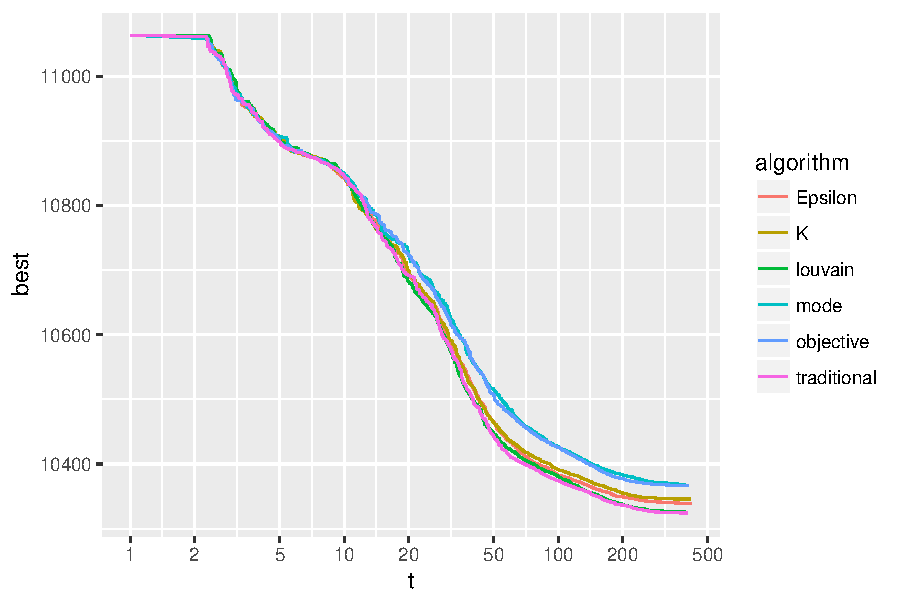
\includegraphics{bachelorarbeit-badcrosscombines}
\end{center}
\end{figure}


\begin{figure}
\caption{Different replacement strategies}
\begin{center}
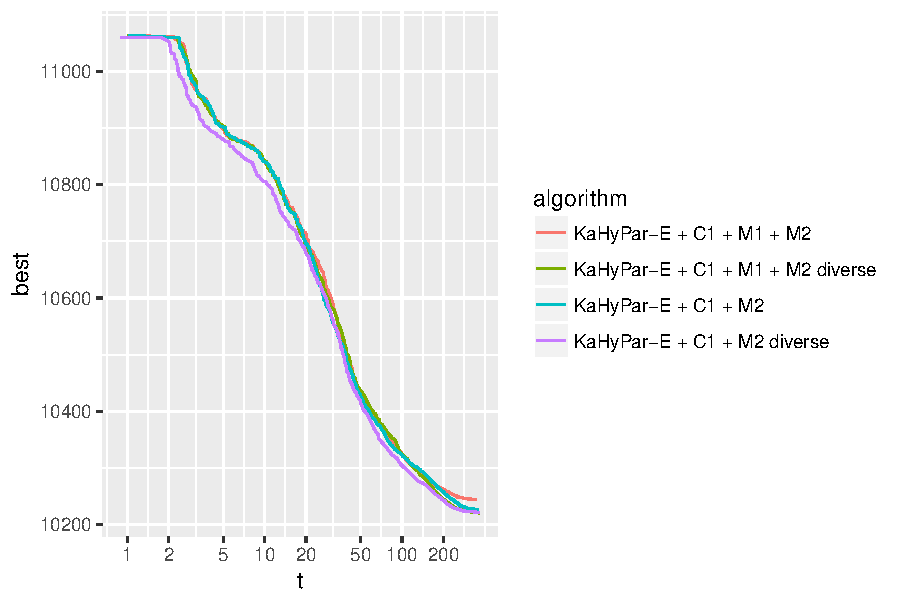
\includegraphics{bachelorarbeit-insertrandom}
\end{center}
TODO replacement strategies can vary 

\end{figure}


%%%%%%%%%%%%%%%%%%%%%%%%%%%%%%%%%%%%%%%%%%%%%%%%%%%%%%%%%%%%%%%%%%%%%%
\chapter{Discussion}
\section{Conclusion}
\section{Future Work}
Vcycles härter
Kreativere auswahlstrategie

\clearpage
\begin{appendix}
\chapter{Implementation Details}
\section{Software}
% Data Structures etc..
\section{Hardware}
\end{appendix}
%%%%%%%%%%%%%%%%%%%%%%%%%%%%%%%%%%%%%%%%%%%%%%%%%%%%%%%%%%%%%%%%%%%%%%
\bibliographystyle{gerplain}
\bibliography{literatur}
\end{document}
